\documentclass[]{report}
\usepackage{graphicx}
\usepackage{tabularx}
\usepackage{multirow}
\usepackage{graphicx}
\usepackage{float}
\usepackage{wrapfig}
\usepackage[export]{adjustbox}
\usepackage[backend=bibtex]{biblatex}
\usepackage[english]{babel}
\usepackage[left=1.25in,top=0.55in,right=0.85in,bottom=0.7in]{geometry}
\addbibresource{bib1}
% Title Page
\title{Rube Goldberg Machine: \\CS251 Project by Group 02}

\author{Harshal ,  Tanmay, \quad Navneet\\140050003  140100011  140100090\\ harshal.m \quad  tanmayb \quad navneet}


\begin{document}
\maketitle
\tableofcontents
\newpage
\chapter{Honour Code}
I pledge on my honour that I have not consulted or given any assistance to any group for this particular project.
\\
I pledge on my honour that I have not consulted or given any assistance to any group for this particular project.
\\
I pledge on my honour that I have not consulted or given any assistance to any group for this particular project.
\chapter{Introduction}
\section{Group Details}
We try to automate every task possible.And we exterminate our problems as they come our way,crushing them like bugs. We are \textbf{The Blitz Exterminators}.
\begin{center}
\begin{tabular}{ |c|c|c|}
\hline
\textbf{Group Name} & \textbf{Roll No.} & \textbf{Name} \\
\hline
\multirow{3}{*}{Blitz Exterminators}& 140050003 & Harshal\\
& 140100011 & Tanmay \\
& 140100090 & Navneet\\
\hline
\end{tabular}
\end{center}
\hfill \break
\section{About Project}
\textbf{Rube Goldberg Machine} is a contraption, invention, device or apparatus that is deliberately over-engineered to perform a simple task in a complicated fashion, usually including a chain reaction. This project is a part of CS 251 course undertaken by second year under graduate students of 2015-2016 in the Autumn Semester

\section{About Topic}
\textbf{Water Server} is a concoction used to interactively serve water to user using various components such as dominos,pulleys,conveyor belt,gates,criss cross structures etc.
\chapter{Interface}
\begin{center}
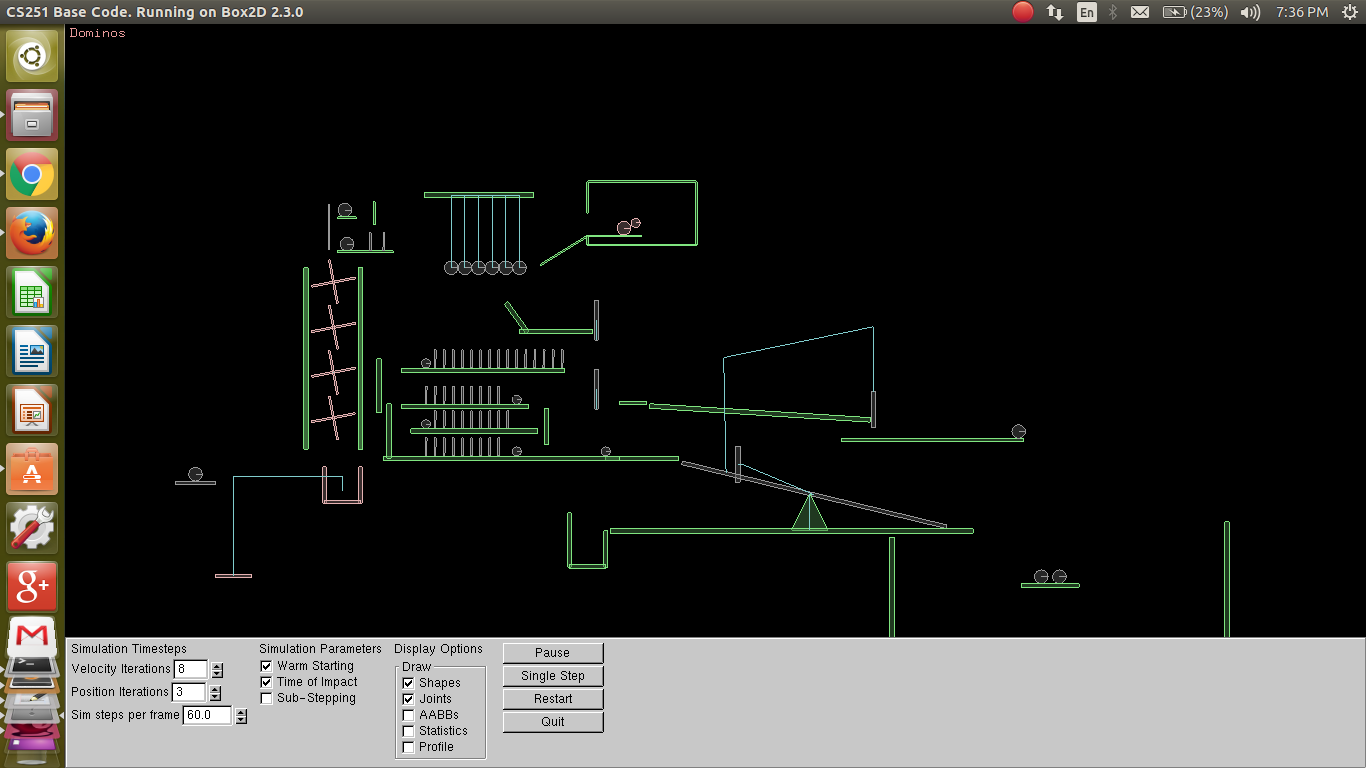
\includegraphics[width=12cm]{img/FirstContact}
\end{center}

\textbf{Instructions}
\begin{itemize}
\item Compile the code using make command at the base folder
\item To run the code run the command "./bin/cs251\_base"
\item To view the documtation view the pdf formed "report.pdf" at the base folder
\item To view the presentation view the pdf "Beamer.pdf" at the base folder
\end{itemize}
\textbf{Buttons}
\begin{itemize}
\item On running the executable you can see a new window popped up. There are a few buttons below using which you can tweak the simulation
\item Pause, Single Step, Restart and Quit control the overall simulation and the window.
\begin{itemize}
\item[\textbf{Pause}:] You can pause the simulation
\item[\textbf{Restart}:] You can restart the simulation
\item[\textbf{Single Step}:] You can proceed the simulation step by step to analyse the processes
\item[\textbf{Quit}:] Quit the window in a safe way
\end{itemize}
\item Other than that there are also Display Options which you can play around with
\begin{itemize}
\item[\textbf{Shape}:] Shows the final outline of the objects displayed 
\item[\textbf{Joints}:] Shows the joints and fixtures(literally) in the simulation frame 
\item[\textbf{AABB}:] Shows the outlining co-ordinates 
\item[\textbf{Statistics}:] Shows the statistics of the processes and functions called
\item[\textbf{Profiling}:] Profiles the callgraphs and the call stack history
\end{itemize}
\item You can also tweak with the Timesteps in the following ways:
\begin{itemize}
\item[\textbf{Velocity Iteration}:] To improve the stability
\item[\textbf{Position Iteration}:] To improve overlap resolution
\item[\textbf{Sim Steps per Frame}:]The Simulation steps happening per frame
\end{itemize}
\end{itemize}
\newpage
\chapter{Deviations}
\section{Changes}
Initially our Project Design was the following
\begin{center}
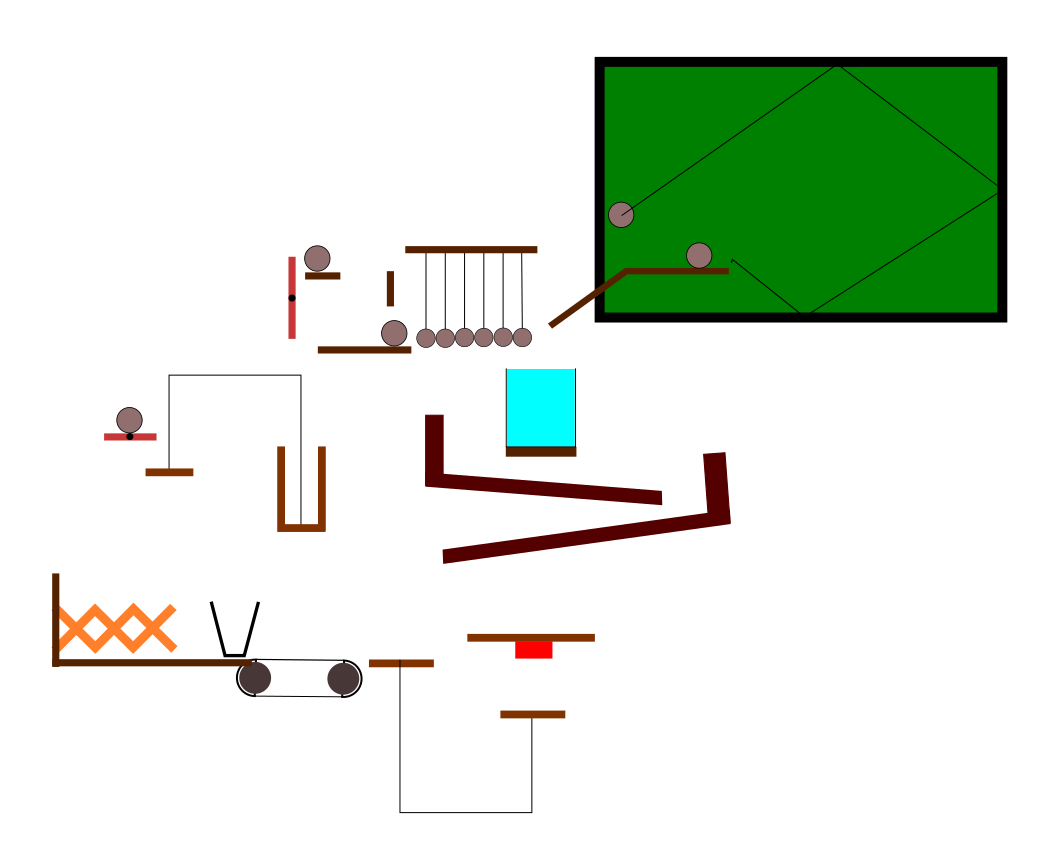
\includegraphics[width=12cm]{img/img}
\end{center}
\begin{itemize}
\item The number of components we had initially seemed less so we decided to increase the components and make it more interactive .
\item Thus we increased the components such as the dominos cycle in the middle and the see saw with the implementation of the gate for obstruction to the ball.
\item Moreover to increase the amount of water collected we went on to implement two containers of fluid instead of one.
\end{itemize}
Finally our project diagram looked like:
\begin{center}
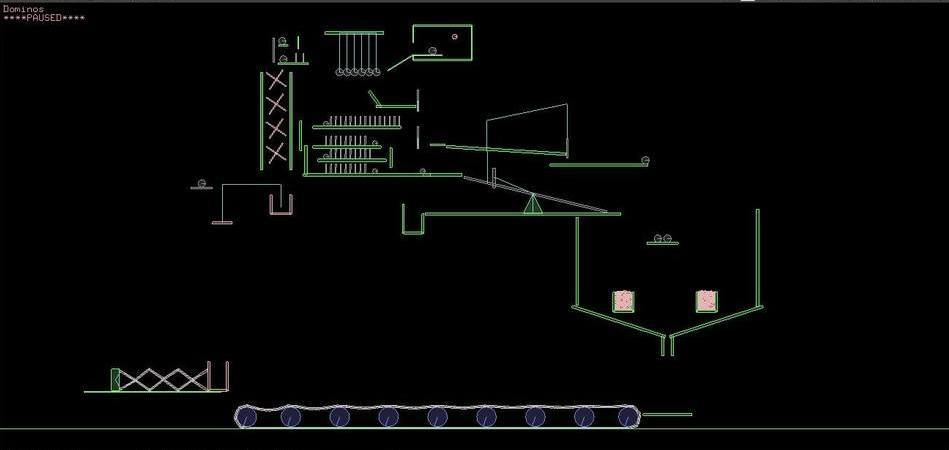
\includegraphics[width=12cm]{img/whole}
\end{center}
\section{Components}
The following Compoonents were used
\begin{enumerate}
\item Dominos
\item  Pulleys
\item  Snooker table
\item Conveyor Belt
\item Newton's Cradle
\item Mills
\item Fluid
\item Criss-cross structure
\end{enumerate}

\newpage
\chapter{Observations}
\begin{center}

\includegraphics[width=15cm]{img/project}
\end{center}
The call graph indicates that many functions have finite amount of time ,however the function b2World::SolveTOI takes the maximum amount of time.Similarly the function b2World::Solve and b2ContactSolver::SolveVelocityConstraints take large amount of time.The max time taking function other than these are b2Vec2::b2Vec2 b2Fixture::IsSensor
\begin{center}
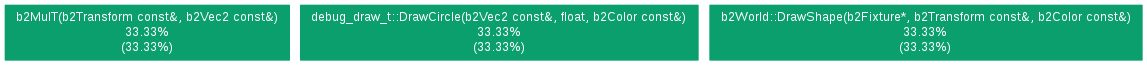
\includegraphics[width=15cm]{img/original}
\end{center}
All the three function b2MulT,debug\_draw\_t:DrawCircle and b2World::DrawShape take approximately equal time that is 0.01 seconds which is lot less compared to the project.This is because of the inclusion of fluids in the project which radically increases the time of the world formation. 
\newpage
\chapter{Working}
\section{Initialization}
\begin{itemize}
\item A snooker ball on the table hits the three sides of the walls finally just bruising the ball giving it enough velocity to initialize the system.
\begin{center}
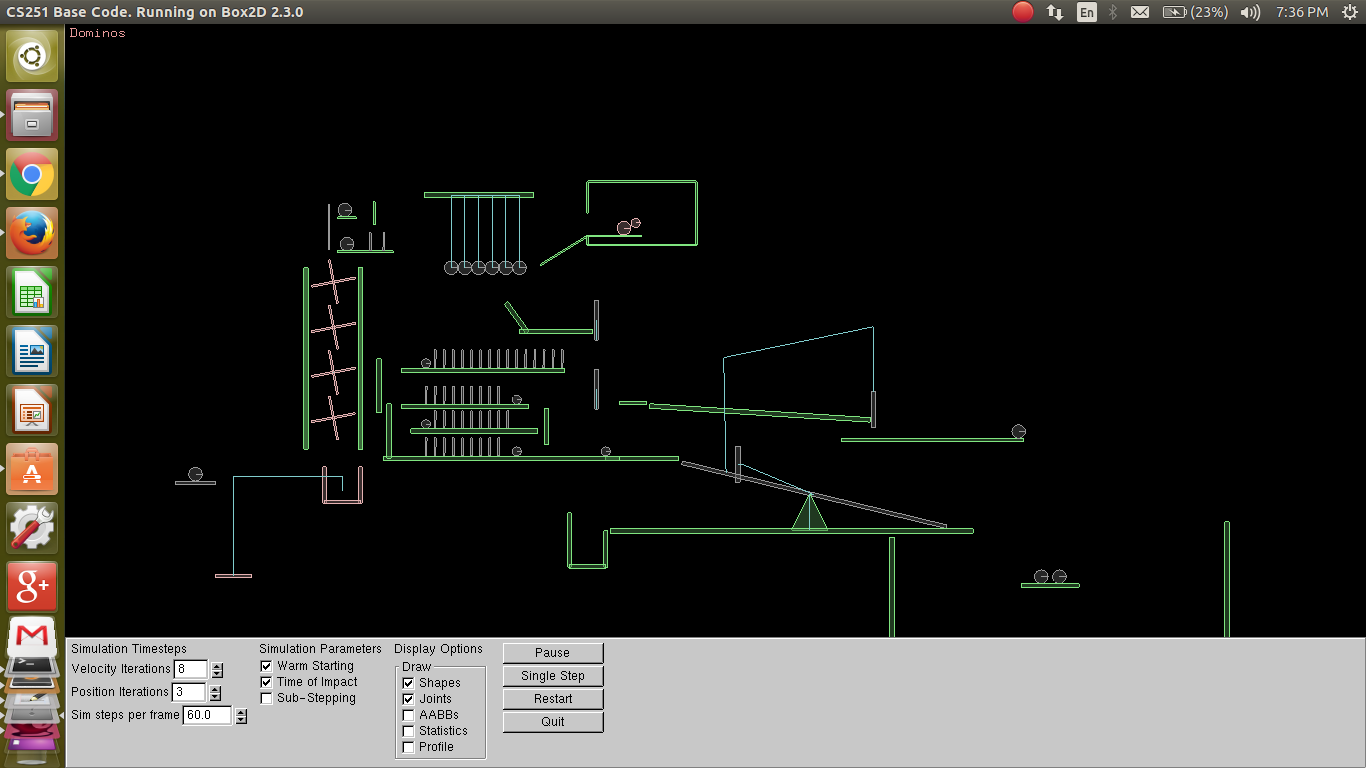
\includegraphics[width=5cm]{img/FirstContact}
\end{center}
\end{itemize}

\section{Setup for Container}
\begin{enumerate}
\item The ball hits the Newtons Cradle which starts a small sequence of Dominos present on the left
\begin{center}
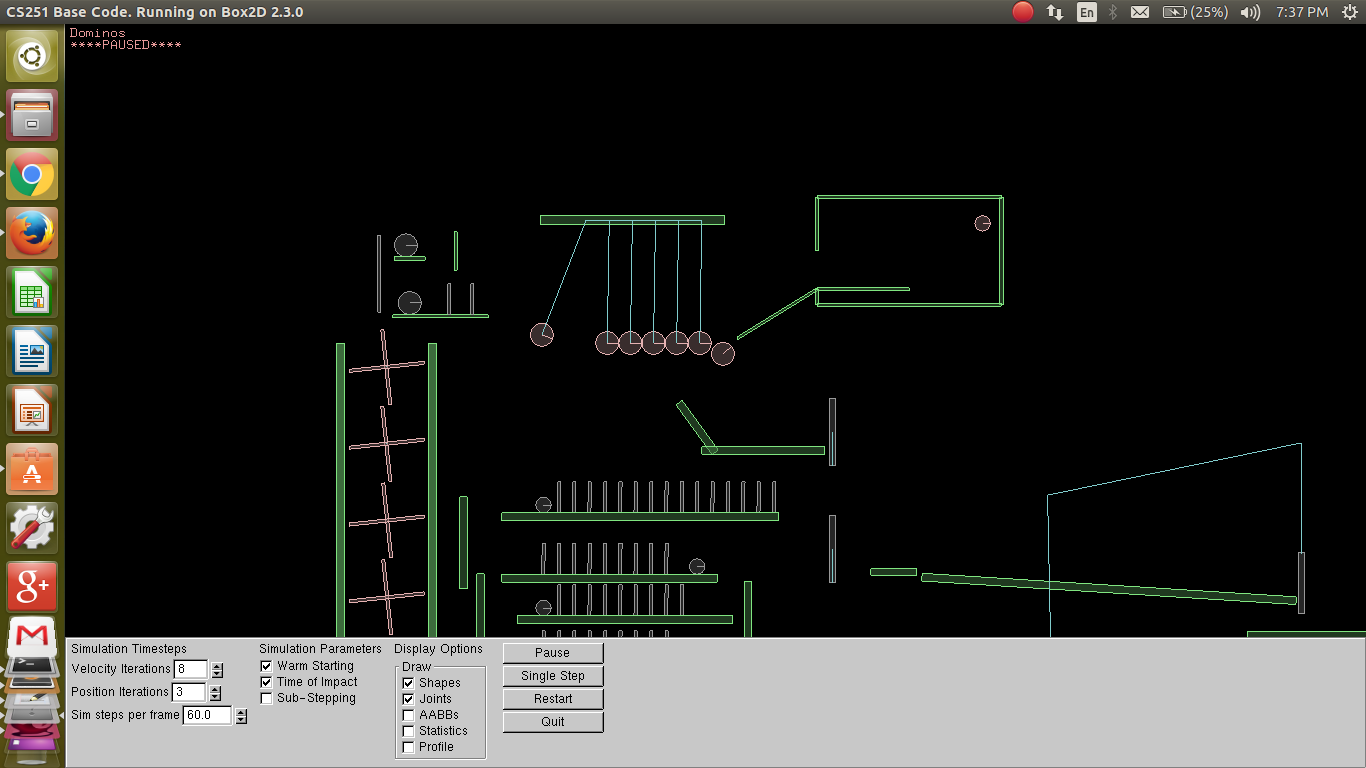
\includegraphics[width=5cm]{img/SecondContact}
\end{center}
\item The dominos hits the ball which hits the vertical plank before falling into the mill causing the second ball to fall into the mill as well
\begin{center}
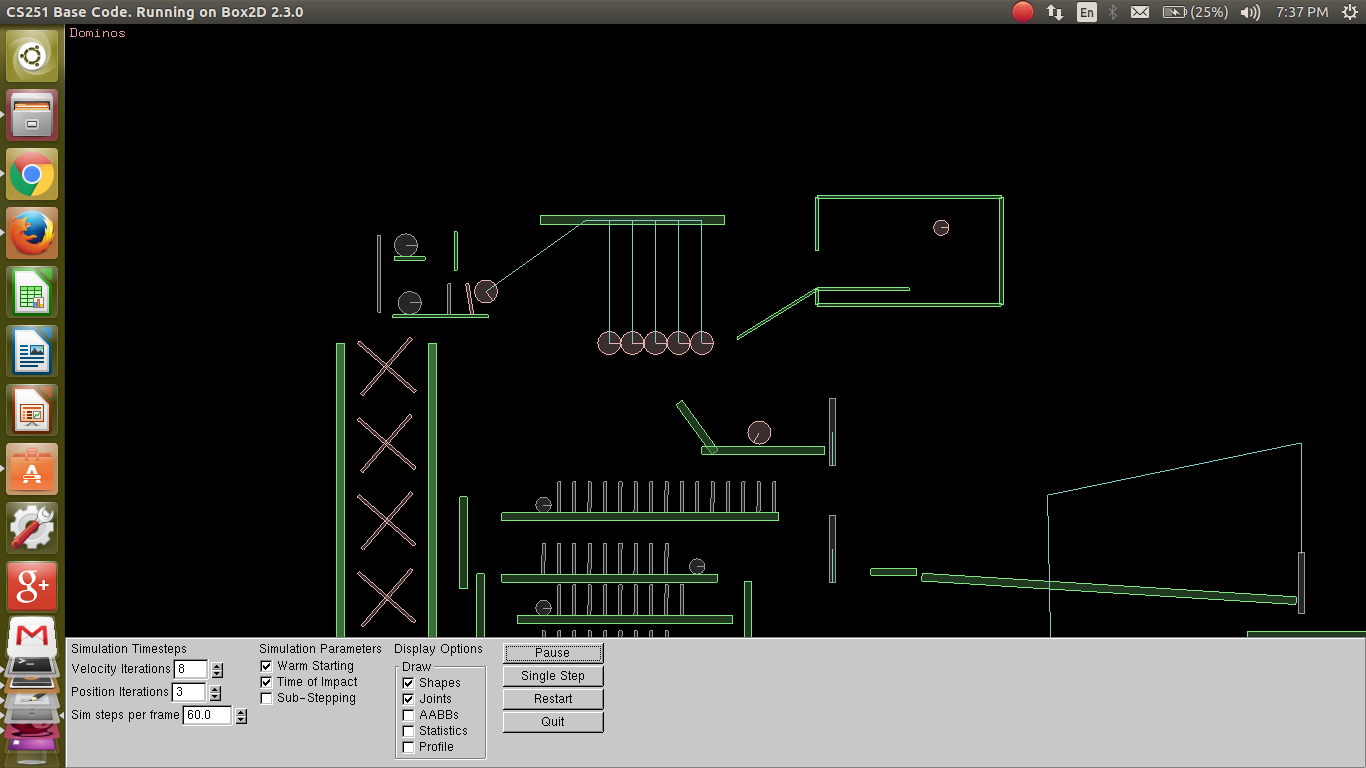
\includegraphics[width=5cm]{img/ThirdContact}
\end{center}
\item The balls fall into the open box which tips the horizontal plank on its downward movement. The heavy ball on the horizontal plank falls on the criss cross structure and the container is pushed on the conveyor belt below
\begin{center}
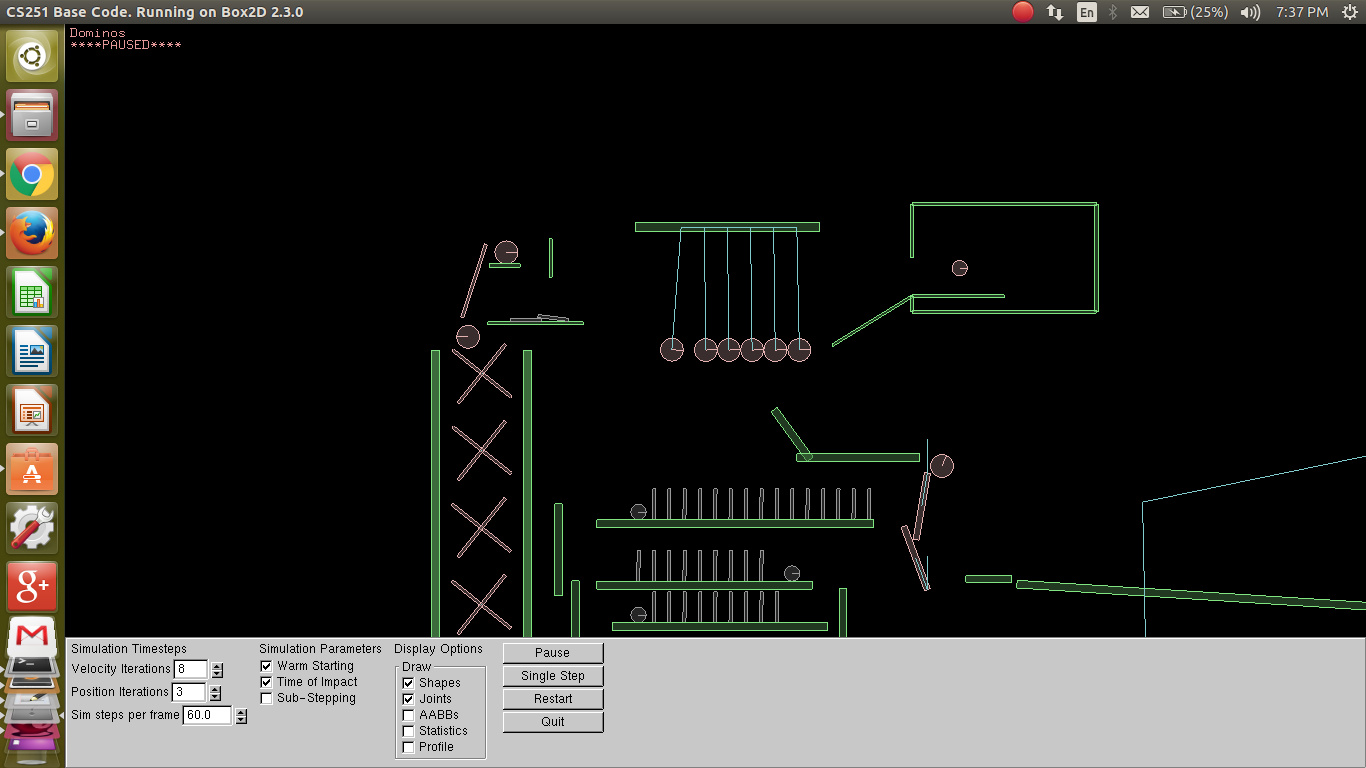
\includegraphics[width=5cm]{img/FourthContact}
\end{center}
\end{enumerate}
	\section{Setup for Pouring Water}
\begin{enumerate}
\item The ball which hits the Newton's Cradle falls down and initializes many sequences of the multi-level dominos sequence
\begin{center}
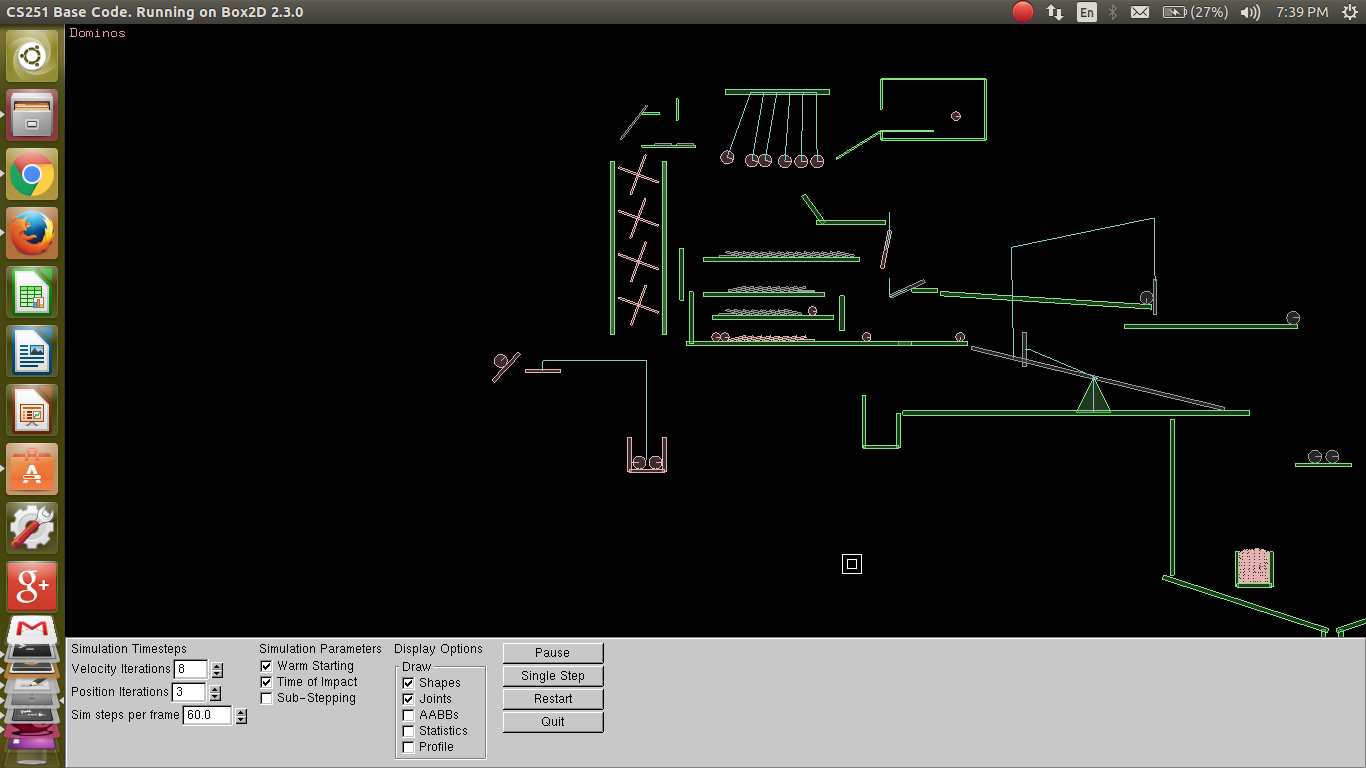
\includegraphics[width=5cm]{img/fifth}
\end{center}
\item The ball later gets obstructed by the gate.
\item The dominos will push the balls onto the seasaw which will initialize the gate at which the ball from the Newton's Cradle was held.  
\item The ball hits another ball tipping it over and later pushes the two balls into the container containing water
\item The overflown water falls into the funnel, which is later collected into the vessel
\end{enumerate}
\newpage
\printbibliography
\nocite{ShareLatex}
\nocite{Box2D}
\nocite{Tutorials_Box2D}
\nocite{Youtube}
\nocite{Github_Conveyor_Belt}
\nocite{General_Problems}
\end{document}          
